% Latex template: https://github.com/mqTeXUsers/Macquarie-University-Beamer-Theme

% Slide Masters:

% Title
% Text
% 2 column
% Full-image
% Bibliography
% Closing
\PassOptionsToPackage{table}{xcolor}    % https://tex.stackexchange.com/a/5365/5483
\documentclass[aspectratio=169, 12pt]{beamer} % Aspect ratio
% https://tex.stackexchange.com/a/14339/5483 
% Possible values: 1610, 169, 149, 54, 43 and 32.
% 169 = 16:9

\usetheme{macquarie}

\usepackage[english]{babel}       % Set language
\usepackage[utf8x]{inputenc}      % Set encoding
\usepackage{colortbl}
\mode<presentation>           % Set options
{
  \usetheme{default}          % Set theme
  \usecolortheme{default}         % Set colors
  \usefonttheme{default}          % Set font theme
  \setbeamertemplate{caption}[numbered] % Set caption to be numbered
}

% Uncomment this to have the outline at the beginning of each section highlighted.
%\AtBeginSection[]
%{
%  \begin{frame}{Outline}
%    \tableofcontents[currentsection]
%  \end{frame}
%}

\usepackage{graphicx}         % For including figures
\usepackage{booktabs}         % For table rules
\usepackage{hyperref}         % For cross-referencing


\setbeamertemplate{footline}[frame number] 

\title{Seven years of FAIMS Mobile} % Presentation title
\author{Shawn A Ross}               % Presentation author
\institute{Office of the Deputy Vice-Chancellor (Research)}         % Author affiliation
\date{\today}                 % Today's date  
\begin{document}

% Title page
% This page includes the informations defined earlier including title, author/s, affiliation/s and the date
% \begin{frame}[noframenumbering]

\maketitle

  
% \end{frame}

% Outline
% This page includes the outline (Table of content) of the presentation. All sections and subsections will appear in the outline by default.
\begin{frame}{Strategies for field recording infrastructure}
  \tableofcontents
\end{frame}

% The following is the most frequently used slide types in beamer
% The slide structure is as follows:
%
%\begin{frame}{<slide-title>}
% <content>
%\end{frame}

\section{Transparency and reproducibility}

\begin{frame}{The 'reproducibility crisis'}
  For nearly a decade the ‘reproducibility crisis’ has featured in the scientific literature \cite{Jasny2011-bw, Baker2016-cf, Munafo2017-bj}. Low reproducibility rates have emerged from large-scale studies:
    \begin{itemize}
        \item Results from only 39\% of psychology studies could be reproduced \cite{Open_Science_Collaboration2015-vf}
        \item Even lower reproducibility rate in biomedical research \cite{Begley2012-xt,Prinz2011-za}
    \end{itemize}
\end{frame}

\begin{frame}{Perceptions of the reproducibility crisis}
  \begin{figure}[H]
    \centering
        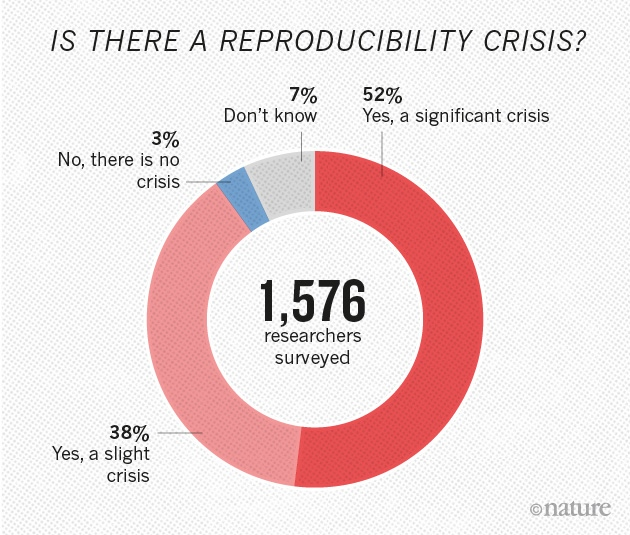
\includegraphics[height=.7\textheight]{figures/reproducibility-graphic-online1.jpeg}
        \caption{Is there a reproducibility crisis? \cite{Baker2016-cf}}
        \label{fig:figure1}
  \end{figure}
\end{frame}

\begin{frame}{The response: improved rigour and transparency}
  'Trust but verify': emerging good practice:
    \begin{itemize}
        \item Findable, Accessible, Interoperable, and Reusable (FAIR) data \cite{Wilkinson2016-mr, Go-fair2017-vs}
        \item Transparency and Openness Promotion (TOP) guidelines \cite{Nosek2015-wm}
        \item Data transparency toolkit \cite{Perkel2018-rw}
    \end{itemize}
\end{frame}

\begin{frame}{The response: from guidelines to mandates}
  Recent mandates for transparency or reproducibility:
    \begin{itemize}
        \item Nature: Transparency Upgrade \cite{Nature2017-lq}
        \item Nature: FAIR data in Earth science \cite{Nature2019-ng}
        \item Copernicus: FAIR data in atmospheric sciences \cite{Van_Edig2018-bu}
        \item Not just the natural sciences: AJPS requires data and code \cite{Jacoby2017-lw, Ajps2015-ex} 
        \item TOP Guidelines have 5000 signatories, including publishers representing 1000 journals (https://cos.io/our-services/top-guidelines/)
    \end{itemize}
\end{frame}

\begin{frame}{TOP Guidelines: publisher adoption}
  \begin{figure}[H]
    \centering
        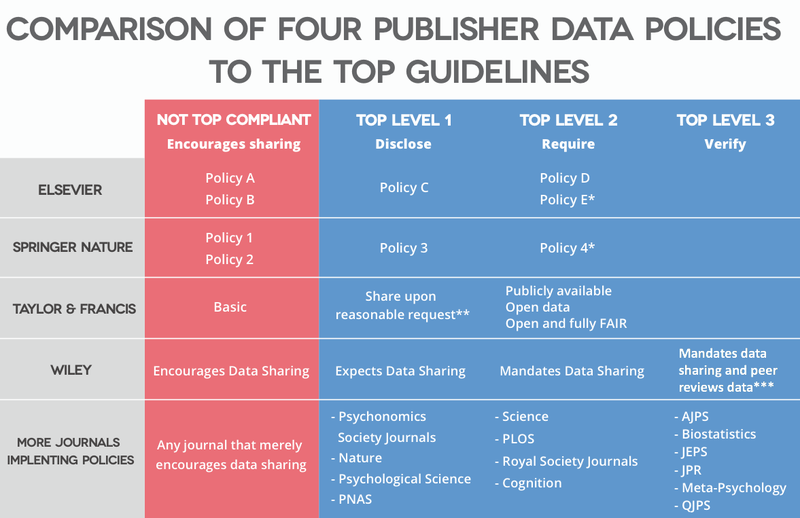
\includegraphics[height=.7\textheight]{figures/TOP-landscape.png}
        \caption{The Landscape of Open Data Policies \cite{Mellor2018-bf}}
        \label{fig:figure1}
  \end{figure}
\end{frame}

\begin{frame}{Level 2 TOP Guidelines for authors (excerpt)}
    \renewcommand{\labelenumii}{\alph{enumii}}
    \begin{enumerate}
        \setcounter{enumi}{1}
        \item Authors using original data must:
            \begin{enumerate}
            \item make the data available at a trusted digital repository [...]
            \item include all variables, treatment conditions, and observations described in the manuscript.
            \item provide a full account of the procedures used to collect, preprocess, clean, or generate the data.
            \item provide program code, scripts, codebooks, and other documentation sufficient to precisely reproduce all published results.
            \item provide research materials and description of procedures necessary to conduct an independent replication of the research.
            \end{enumerate}
    \end{enumerate}
    Source: https://osf.io/edtxm/
\end{frame}

\begin{frame}{What does this mean? Are we ready?}
  In practice, emerging good practice - and policies from publishers and funders - mean that:
    \begin{itemize}
        \item Comprehensive, FAIR datasets will be deposited in domain-specific repositories. Data, and especially metadata, quality will be higher.
        \item Data will be captured digitally as early in research as possible, and provenance / version history maintained.
        \item Research approach, processes, and procedures will be documented.
        \item Data processing and analysis will use code (not Excel or ARCGIS!) 
        \item Code will be documented and published for reuse.
        \item Further steps taken for analytical reproducibility (use of OSS, version control, automation, containerisation, etc.). 
    \end{itemize}
\end{frame}

\begin{frame}{Beyond compliance: large-scale, synthetic research}
  The same approaches that facilitate transparency and reproducibility support the kind of scalable research that can address archaeological 'grand challenges' \cite{Kintigh2014-u}:
\end{frame}

\section{Infrastructure across the data lifecycle}

\begin{frame}{Context: the challenge of 'small data'}
    'Long tail' research: most field data is small data \cite{Borgman2015-rh}
      \begin{itemize}
        \item Smaller scale; smaller communities; local control.
        \item Diverse questions, approaches, and methods.
        \item Heterogeneous data; variety of content, structure.
        \item Data and infrastructure emerge from fieldwork. 
        \item Relative lack of standards.
        \item Limited infrastructure and funding.
        \item Challenges associated with big(ger) data from photogrammetry, SfM, video, geophysics, etc., will exacerbate these problems.
    \end{itemize}
\end{frame}

\begin{frame}{Infrastructure across the data lifecycle}
    Consider the infrastructure needed to manage the three main phases of the data lifecycle
      \begin{itemize}
        \item Publication (easiest): domain-specific repositories.
        \item Processing and analysis (harder): project-level code \cite{Stewart_Lowndes2017-lj} then Virtual Labs / Science Gateways.
        \item Capture (hardest): most varied, needs to work offline under difficult conditions.
    \end{itemize}
\end{frame}

\section{Lessons from FAIMS}

\begin{frame}{Introduction to the FAIMS Project}
      \begin{itemize}
        \item The Field Acquired Information Management Systems (FAIMS) Project began in 2012 as an information infrastructure project for field data capture in archaeology.
        \item Developed FAIMS Mobile, a generalised, customisable platform \cite{Ballsun-Stanton2018-zd}.
        \item Use expanded beyond archaeology to geoscience, ecology, ethnography, linguistics, oral history
        \item Has been customised for over 50 workflows at more than 30 projects. 
        \item Data and workflow modelling for these customisations has provided unique insights into field data capture and the infrastructure needed to support it.
    \end{itemize}
\end{frame}

\begin{frame}{Key aspects of FAIMS Mobile}
    Field data capture infrastructure
      \begin{itemize}
        \item We deserve research-specific software.
        \item Diverse practices and limited resources require generalised software.
        \item Do one thing well with modular and federated software (but slice the pie carefully).
        \item Open-source software has advantages (but is difficult to sustain). 
        \item Scope requirements carefully.
        \Item Invest in outreach and engagement.
    \end{itemize}
\end{frame}

\begin{frame}{Research specific}
    Archaeology needs (and deserves) research-specific software, contra \cite{Roosevelt2015-kd}.
      \begin{itemize}
        \item Most commercial / mass-market software does not meet research needs.
        \item Risk of lock-in, unwelcome changes to features or business models, and product discontinuation.
    \end{itemize}
\end{frame}

\begin{frame}{Generalised}
   Commercial software doesn't meet our needs, and bespoke development is too expensive and usually unsustainable.
      \begin{itemize}
        \item Generalised software can be deeply customised to accommodate our diverse data types, data models, workflows, etc.
        \item The code used to customise it describes the data model and workflow.
        \item Customisations can be published and re-deployed trivially.
        \item Can deliver research-grade software affordably.  
    \end{itemize}
    FAIMS Mobile cost perhaps 3x a single bespoke application, but has been customised 50x. Customisation cost is 1/10th bespoke, and still <1/2 even if 'core' platform development costs are amortised across projects.
\end{frame}

\begin{frame}{Modular and federated}
   Do one thing well.
      \begin{itemize}
        \item Identify other infrastructure in the domain and interoperate with it (via ETLs or APIs).
        \item It is better to divide by data-lifecycle phase rather than data type, since our data is so integrated.
    \end{itemize}
\end{frame}

\begin{frame}{Open source?}
   Open source has advantages but is difficult to sustain.
      \begin{itemize}
        \item Emerging open research principles strongly prefer OSS as opposed to proprietary ‘black boxes’.
        \item Transparency and reusability (esp. customisation code).
        \item Ability to hand off from one organisation to another (esp. 'core' platform code).
        \item Ability to fork code prevents lock-in and mitigates unwelcome decisions by software developers.
        \item BUT OSS business models are hard to scale and rely on occasional injections of grant or institutional funding.
    \end{itemize}
\end{frame}

\begin{frame}{Scope carefully}
   Seek facts not opinions.
      \begin{itemize}
        \item Don’t ask researchers what they think, ask them what they have done - what software they have adopted and why, and what problems they have expended resources to solve. 
        \item ‘Lean startup’ methodology very useful (based around interviews with potential users).
        \item In our case, we over-invested in mobile GIS and under-invested in usability (especially a GUI for customisation).
    \end{itemize}
\end{frame}

\begin{frame}{Spend on outreach and engagement}
   If you build it they will not come; people can't use technologies they don't know about.
      \begin{itemize}
        \item As per industry standards, dedicate at least 30\% of any information infrastructure budget to outreach and engagement (sales and marketing). 
        \item Typical academic outreach (journal articles, conference presentations, workshops, even booths at major conferences) are not enough.
    \end{itemize}
\end{frame}

\begin{frame}{FAIMS publications}
      \begin{itemize}
        \item \cite{Sobotkova2018-al}
        \item \cite{Ballsun-Stanton2018-zd}
        \item \cite{VanValkenburgh2018-hv}
        \item \cite{sobotkova2016-mx}
        \item \cite{Ross2015-ph} 
        \item \cite{Sobotkova2015-lq}
        \item \cite{Ross2013-hi}
    \end{itemize}
\end{frame}

\section{From current practice to better practice}

\begin{frame}{Challenges and paths forward}
   How do we get from where we are now to where we want to be?
      \begin{itemize}
        \item Understand the evolving expectations of transparent research. 
        \item Look past desktop software (Excel, ARCGIS, Filemaker, Access, etc.).
        \item Rally around emerging research- and domain-specific solutions (even if you are only 80\% happy with them).
        \item Overcome 'not invented here'; you don't need a bespoke solution.
        \item Budget for 'ground-up' transparency (data and code). Understand that up-front costs (in time and money) will be high but offer longer-term payoffs (in costs, time, and quality).
        \item De-emphasise 'sharks with laser beams'; budget for fundamental good practice in data and code management before other technologies (you need it more than photogrammetry, drones, etc.).
    \end{itemize}
\end{frame}

% Adding the option 'allowframebreaks' allows the contents of the slide to be expanded in more than one slide.
% The "1" comes from the outer theme"
\begin{frame}[allowframebreaks]{References}
  \tiny
  \bibliography{references}
  \bibliographystyle{apalike}
\end{frame}


\begin{frame}[standout]
Thank you!
\end{frame}



\end{document}
